%Spring 2018 Euclidean Handout 
\documentclass{tufte-handout}

%\geometry{showframe}% for debugging purposes -- displays the margins

%%%% Packages to make things pretty
\usepackage{amsmath,amsthm}
\usepackage{booktabs}
\usepackage{graphicx}
\setkeys{Gin}{width=\linewidth,totalheight=\textheight,keepaspectratio}
\graphicspath{{graphics/}}
\usepackage{units}
\usepackage{fancyvrb}
\fvset{fontsize=\normalsize}
\usepackage{multicol}
\usepackage{pdfpages}

%%%% Theorem Evironments
\theoremstyle{definition}
\swapnumbers
\newtheorem{problem}{Problem}[section]
\newtheorem{conjecture}[problem]{Conjecture}
\newtheorem*{definition}{Definition}
\newtheorem*{theorem}{Theorem}
\newtheorem{question}[problem]{Question}
\newtheorem{challenge}[problem]{Challenge}
\newtheorem*{postulate}{Postulate}

%%%%%


\title{Euclidean Geometry:\\An Introduction to Mathematical Work}
\author[Math 3600]{Math 3600}
\date{Spring 2018}

\begin{document}

\maketitle

\begin{marginfigure}
    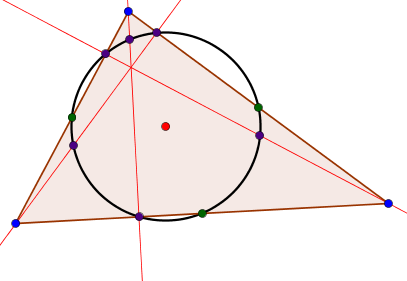
\includegraphics{NPC}
\end{marginfigure}

\section*{Conclusion}


Now the semester comes to a close, and so does our time to study Euclid and the subject he helped organize and promote. It was important to me that you learn to ``stand on your own two feet" when doing mathematics, and so I asked you not to use any other references during our class. The time for that to end has also come. At this point, you should be ready to read widely in geometry as an engaged and active participant.\\

But what might you read? Since Euclid's time geometry has exploded into a vast and varied subject. \marginnote{You might also consider studying some of these: \emph{projective geometry}, \emph{hyperbolic geometry}, \emph{solid geometry}, \emph{combinatorial geometry}, \emph{discrete geometry}, \emph{computational geometry}, etc.

There is another branch of mathematics called \emph{topology} that has geometry as one of 
its parents. That is pretty neat, too.}
In the hands of Ren\'{e} Descartes and Pierre de Fermat geometry was married to algebra, this in turn prepared the way for The Calculus of Leibniz and Newton. 
Using algebra to study geometry is a subject now called \emph{Algebraic Geometry}, and using (multi-variable) calculus to study geometry is called \emph{Differential Geometry}.  Spectacular things are now happening in both of these major branches of geometric study, and if you'd like to learn some more, ask me for some guidance. 
\marginnote{There is a highly abstract field called \emph{Category Theory} which is lately making an exciting attempt to discuss ``spaces'' under the name of \emph{higher geometry}!}
Of course, these aren't entirely separate, and they don't cover all of what is happening in modern geometric inquiry.\\

Not many people actively pursue the study of planar geometry in Euclid's footsteps these days, but that doesn't mean that the subject is ``dead.'' On the contrary, mathematics students use it as we have used it: as a playground for learning to do mathematics and gaining power. This is still true in most High School curricula to some extent. I didn't seriously study this material until a few years ago when I realized I was going to teach it, and its charms have won me over. If you have been similarly inspired this semester, be cheered that there is a lot more of this classical stuff: we have barely scratched the surface. Perhaps you will be interested in the following books for further study:

\begin{description}
\item[Pedoe, Daniel] \emph{Geometry: a Comprehensive Course}, Dover Publications, 1988. \marginnote{ISBN-13: 978-0486658124}
\end{description}

This book and any book by Dan Pedoe are heartily recommended.

\begin{description}
\item[Hartshorne, Robin] \emph{Geometry: Euclid and Beyond}, Springer, 2000. \marginnote{ISBN-13: 978-0387986500}
\end{description}

This book was the inspiration for the course you just took. In it, Hartshorne takes a semi-historical approach, starting with a critical reading of Euclid. He then builds up some modern marvels, mostly vindicating Euclid's ideas along the way.

\begin{description}
\item[Kiselev, A. and Givental, A.] \emph{Kiselev's Geometry: Book I. Planimetry}, Sumizdat, 2006. \marginnote{ISBN-13: 978-0977985203}
\end{description}

This book is a classic of the Russian school mathematics tradition. It was used for decades in the USSR as the standard grade school planar geometry book. 
\marginnote{A bonus: the introduction has a really good rant about the state of US geometry education!} 
It is essentially a good reworking of Euclid, with some more modern concepts thrown in, adapted for school use. 
There is a second book on spatial geometry, but I haven't looked at it enough, yet, to recommend it.

While I have your attention, I want to point out two books that were standard college-level geometry textbooks a few generations ago, when everyone who succeeded at high school geometry got the firm grounding you have now. If you want to get your hands dirty again and learn some pretty theorems, this is a place to start. 

\begin{description}
\item[Altschiller-Court, Nathan] \emph{College Geometry: An Introduction to the Modern Geometry of the Triangle and the Circle}, Dover Publications, 2nd revised and enlarged edition, 2007. \marginnote{ISBN-13: 978-0486458052}

\item[Johnson, Roger A.] \emph{Advanced Euclidean Geometry}, Dover Publications, 2007.\marginnote{ISBN-13: 978-0486462370}

\end{description}

And finally, I love this interesting book about the history of geometry. From it, you can learn some history and a lot of mathematics.

\begin{description}
\item[Gray, Jeremy] \emph{Worlds out of Nothing: A Course in the History of Geometry in the 19th Century}, Springer, 2010
\marginnote{ISBN-13: 978-0857290595}
\end{description}

There are certainly many other good books out there. Go explore.\\

\noindent\textit{ps.} You might also consider taking the other geometry courses offered at UNI: 
\begin{itemize}
\item MATH 4600 \emph{Geometric Transformations}, 
\item MATH 3610 \emph{Modern Geometries},
\item MATH 3630 \emph{Differential Geometry}.
\end{itemize}

\end{document}
